\documentclass{article}
\usepackage[utf8]{inputenc}

\usepackage{geometry}
\geometry{
    textwidth = 18cm,
    footnotesep = 2cm,
    bottom = 3.25cm,
}
\usepackage[strict]{changepage}
\usepackage[document]{ragged2e}
\usepackage[unicode]{hyperref}
\usepackage{amsmath}
\usepackage{graphicx,caption}
\graphicspath{ {./Images/} }
\usepackage{float}
\usepackage[nottoc,numbib]{tocbibind}
\usepackage{xcolor}
\usepackage{fixltx2e}
\usepackage{systeme}
\usepackage{listings}
 
\definecolor{codegreen}{rgb}{0,0.6,0}
\definecolor{codegray}{rgb}{0.5,0.5,0.5}
\definecolor{codepurple}{rgb}{0.58,0,0.82}
\definecolor{backcolour}{rgb}{0.95,0.95,0.92}
 \lstdefinestyle{mystyle}{
    backgroundcolor=\color{backcolour},   
    commentstyle=\color{codegreen},
    keywordstyle=\color{magenta},
    numberstyle=\tiny\color{codegray},
    stringstyle=\color{codepurple},
    basicstyle=\ttfamily\footnotesize,
    breakatwhitespace=false,         
    breaklines=true,                 
    captionpos=b,                    
    keepspaces=true,                 
    numbers=left,                    
    numbersep=5pt,                  
    showspaces=false,                
    showstringspaces=false,
    showtabs=false,                  
    tabsize=2
}
\lstset{style=mystyle}

\newcommand*{\defeq}{\stackrel{\text{def}}{=}}
\newcommand{\newbowtie}{\mathrel{\ooalign{$\triangleright$\,\cr\,$\triangleleft$}}}
\renewcommand*\contentsname{Table of Contents}
\newcommand{\blank}[1]{\hspace*{#1}\linebreak[0]}

\title{Formal Methods Project}
\author{Fabio Dainese (857661), Martina Donadi (865737)}
\date{November 2019}

\begin{document}
\begin{titlepage}
    \begin{center}
      \vspace{2.5cm}\Huge\textbf{Formal Methods for System Verification Project Documentation}\\
      \vspace{2cm}
      \LARGE\textit{A dynamic server allocation for energy efficiency}\\
      \vspace{2cm}\hspace{1cm}\Large\textbf{Martina Donadi, 865737 \hfill Fabio Dainese, 857661}\blank{1cm}\\
      \vspace{1.75cm}\Large\textit{Ca’ Foscari, University of Venice}\\
      \vspace{0.75cm}\Large December 1, 2019\\
      \vspace{3cm}\large\textit{\textbf{Keywords}: PEPA Language, Continuous Time Markov Chain, Server Power Consumption}
   \end{center}
   \let\thefootnote\relax\footnote{\textbf{Fabio Dainese} (email: \href{mailto:857661@stud.unive.it}{857661@stud.unive.it}), \textbf{Martina Donadi} (email: \href{mailto:865737@stud.unive.it}{865737@stud.unive.it}) - Master degree in 'Software Dependability and Cyber Security' (\href{www.unive.it}{www.unive.it}).}
\end{titlepage}

\tableofcontents
\newpage

%%%%%%%%%%% 1 INTRODUCTION %%%%%%
\justifying
\section{Introduction}
Power consumption in data centers receive a huge concern by data centre providers and that's why in this project we are going to model a policy, in PEPA language, that it will dynamically perform the powering on or off of the servers in order to minimize the power consumption according to the demand.\newline

\par\noindent The system taken into consideration consists of a given number (N) of homogeneous servers. These servers may be in any of the following five states:

\begin{itemize}
    \item Powered up (wherein the server may be either active or idle);
    \item Powering up;
    \item Powered down;
    \item Powering down;
    \item Fault.
\end{itemize}

In the transitional conditions, i.e. \textit{powering down} or \textit{powering up}, and the \textit{fault} condition, servers are unable to respond to service demands.\newline
Although the \textit{fault} condition could occur simultaneously with any of the other
four conditions, in this case it's considered only in the transitional
states (\textit{powering up} and \textit{powering down}) due to the increased likelihood of
faults becoming apparent then.\newline

\par\noindent There exists various types of heuristics that are used to organise the servers usage according to the demand, but in this paper we're considering only the 'High/Low' one.\newline
This type of heuristic takes into consideration the arrival periods, switching time, processing time
and the queue length. Furthermore, we assume that the system is very stable, meaning that the jobs' arrival rates are categorized in \(\lambda_{high}\) or \(\lambda_{low}\) binary form and that the jobs time/duration had a fixed value of \(\mu\).\newline
The high/low is a sophisticated heuristic which incorporates the system performance and stability into its definition.\newline

\par\noindent The PEPA model considered in this paper is the one described in \cite{projectPaper} and can basically be regarded as a multi-server queue.

\subsection{Multi-Server Queue Model}
Variation in service and arrival rates causes queues. The problem of minimizing power consumption in data centres can be related to the one of modelling a queue to provide quality of service minimizing costs.
In order to model a queue at least three parameters are necessary:

\begin{itemize}
    \item Arrival rate : how fast a customer is showing up to reach a server in the data center;
    \item Service rate (\(\mu\)) : how fast a server can handle a customer's request;
    \item Number of servers.
\end{itemize}

\begin{figure}[H]
    \centering
    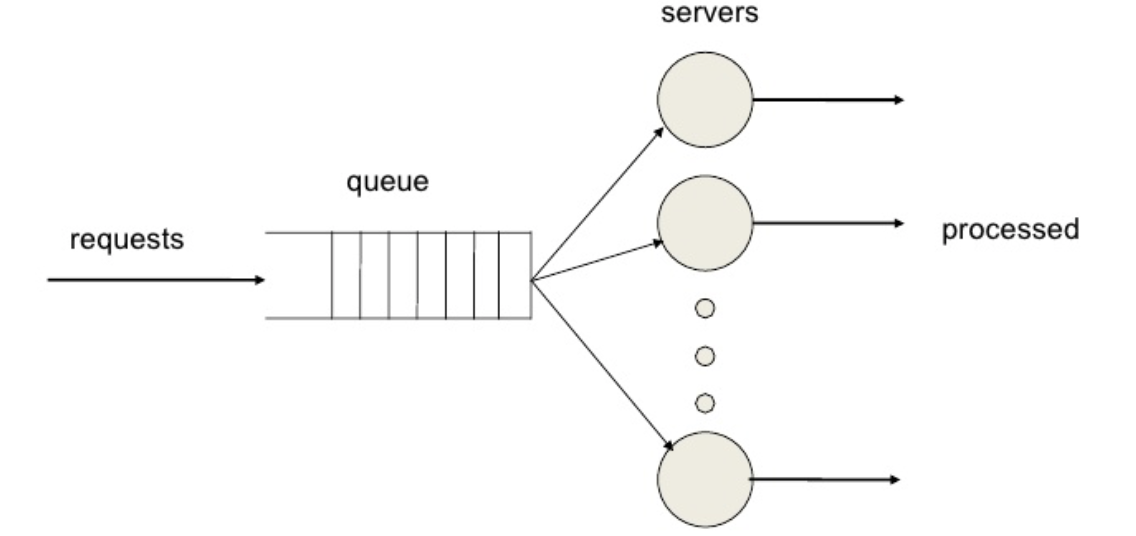
\includegraphics[width=1.0\textwidth]{multi-server-queue.png}
    \caption{Multi server queue}
    \label{fig:multi-server-queue}
\end{figure}

\par\noindent For our model the number of servers is considered to be varying and bounded at N as well as the maximum number of jobs (i.e. the maximum number of customers in the queue) is bounded at N. The arrival rate of jobs in the system is varying: jobs arrive at either a high rate (\(\lambda_{high}\)) or at a low rate (\(\lambda_{low}\)). The service rate is varying according to the number of active servers: M servers out of the N are supposed to be static, i.e. to remain permanently active.
When the queue is not full it engages in an arrival activity (with high/low rate of arrival depending on the current arrival rate of the system). When the queue is full the arrival process is suspended and jobs are lost. When there are \(i\) jobs (\(0 < i \leq N\)) in the queue, it engages in a serve activity at rate \(i*\mu\).\newline

\par\noindent In the following section the model is analyzed in details in terms of components, activities, PEPA representation and problems associated with it.

%%%%%%% 2 COMPONENTS OF THE SYSTEM %%%%%%%%%%%%
\section{Components and Activities of the System}

\subsection{Components of the System}
As we already mentioned before, the model taken into consideration uses a variant of the high/low policy, in which we have \(M\) static servers that remain permanently available to serve jobs, meanwhile the remaining servers might be turn on and off in response to the high and low periods of jobs' arrivals (\(M - N\) servers).\newline

\par\noindent The system will be composed by the following components: 

\begin{itemize}
    \item \(Q_{i}\): Queue's current state, with \(0\leq i \leq N\), which represent the number of jobs in the system at the time \textit{i};
    \item \(Arrival_{high}\), \(Arrival_{low}\): Represent the two possible jobs' arrival stream states (high or low);
    \item All the possible server's state are represented by:
    \begin{itemize}
        \item \(Server_{on}\): State in which the server is either active or idle;
        \item \(ServerPowering_{on}\): State in which the server is turning on;
        \item \(Server_{off}\): State in which the server if fully turned off;
        \item \(ServerPowering_{off}\): State in which the server is turning off;
        \item \(Server_{failOn}\): State in which the server encountered an error performing the power-up activity;
        \item \(Server_{failOff}\): State in which the server encountered an error performing the shutdown activity;
        \item \(Server_{static}\): State representing a server that is always active (\(M\) servers).
    \end{itemize}
\end{itemize}

\subsection{Activities of the System}
In this section we will describe all the possible behaviours, i.e. activities, that each component of the system can perform.

\subsubsection{Activities of the Queue}
The set of possible actions that the \textit{queue} component can perform are:

\begin{itemize}
    \item \textbf{Service}: When a request is successfully elaborated and the job leave the system (at a fixed rate of \(\mu\));
    \item \textbf{arrivalH}: When the arrivals into the system occurs at high rate \(\lambda\);
    \item \textbf{arrivalL}: When the arrival into the system occurs at low rate \(\epsilon\).
\end{itemize}

\subsubsection{Activities of the Arrival Stream}
The activities of the \textit{arrival stream},  identified by the components \(Arrival_{high}\) and \(Arrival_{low}\), are modeled by the previously defined queue activities, i.e. \textbf{arrivalH} and \textbf{arrivalL}, and also by the switching actions between the high and low rate defined through the activities:

\begin{itemize}
    \item \textbf{highPeriodEnd} at rate \(\beta\);
    \item \textbf{lowPeriodEnd} at rate \(\gamma\).
\end{itemize}

\subsubsection{Activities of the Server}
The activities of the server are modeled by the previously defined activities \textbf{highPeriodEnd}, \textbf{lowPeriodEnd}, \textbf{service} and by new ones, such as:

\begin{itemize}
    \item \textbf{powerup}: Used to turn on a server (\(\eta\) rate);
    \item \textbf{poweroff}: Used to turn off a server (\(\xi\) rate);
    \item \textbf{repair}: Used to fix the server in case of error/fault (\(\sigma  rate\));
\end{itemize}

%%%%%%%%%% 3 INTERACTION BETWEEN COMPONENTS %%%%%%%%%%%%
\section{Interactions Between the Components}

To sum up the various behaviours of the previously described components, we can say that the:

\begin{itemize}
    \item \textbf{Queue} will accept the incoming jobs, regardless the type of arrival, up until the queue if full (\(i \leq n\)), plus every time a job is served the queue index counter is decreased by 1;
    \item \textbf{Arrival Stream} will be in charge of detecting and switching accordingly to the appropriate arrival rate stream situation (high or low);
    \item \textbf{Server} will power-up or down accordingly to the high or low jobs arrival. To keep in mind that we have considered also \(M\) static servers.
\end{itemize}

\noindent The interaction between these components are governed by some common activities in which they have to cooperate, such as:

\begin{itemize}
    \item \textbf{Arrival\textsubscript{high}} and \textbf{Server\textsubscript{on}} whenever the '\textit{highPeriodEnd}' activity is performed (moving respectively the system states to \textbf{Arrival\textsubscript{low}} and \textbf{ServerPowering\textsubscript{off}});
    \item \textbf{Arrival\textsubscript{low}} and \textbf{Server\textsubscript{off}} whenever the '\textit{lowPeriodEnd}' activity is performed (moving respectively the system states to \textbf{Arrival\textsubscript{high}} and \textbf{ServerPowering\textsubscript{on}});
    \item \textbf{Arrival\textsubscript{high}/Arrival\textsubscript{low}} and \textbf{Q\textsubscript{i}} whenever the '\textit{arrivalH/arrivalL}' activities are performed (moving respectively the system state to \textbf{Q\textsubscript{i+1}} and remaining to the corresponding \textbf{Arrival\textsubscript{high}/Arrival\textsubscript{low}} state);
    \item \textbf{Server\textsubscript{on}} and \textbf{Q\textsubscript{i}} whenever the '\textit{service}' activity is performed (moving respectively the system states to \textbf{Server\textsubscript{on}} and \textbf{Q\textsubscript{i-1}});
\end{itemize}

\noindent The rest of the activities will change the system's states as follows:

\begin{itemize}
    \item \textbf{Server\textsubscript{static}} will always perform the '\textit{service}' activity and remains in its state;
    \item Whenever \textbf{ServerPowering\textsubscript{on}} will perform the '\textit{powerup}' activity it has a probability \(\rho\) of encountering a problem/fail that will lead it to the state \textbf{Server\textsubscript{failOn}} (and therefore it has the probability of \((1-\rho)\) to perform correctly the activity leading it to the state \textbf{Server\textsubscript{on}});
    \item Whenever \textbf{ServerPowering\textsubscript{off}} will perform the '\textit{poweroff}' activity it has a probability \(\rho\) of encountering a problem/fail that will lead it to the state \textbf{Server\textsubscript{failOff}} (and therefore it has the probability of \((1-\rho)\) to perform correctly the activity leading it to the state \textbf{Server\textsubscript{off}});
    \item Whenever the system is in the \textbf{Server\textsubscript{failOn}}/\textbf{Server\textsubscript{failOff}} state it can only perform the '\textit{repair}' activity, moving it to he corresponding \textbf{Server\textsubscript{on}}/\textbf{Server\textsubscript{off}} state.
\end{itemize}

\noindent A more detailed and formal description of the interactions between the components will be presented in the next section.

%%%%%%%%%%% 4 PEPA COMPONENTS OF THE SYSTEM %%%%%%%%
\section{PEPA Components of the System}

\subsection{Queue PEPA Component}

The \textit{Queue} PEPA component of the system is defined as follows:

\begin{align*} 
    Q_{0} &\defeq (arrivalH, \lambda).Q_{1} + (arrivalL, \epsilon).Q_{1} \\
    Q_{1} &\defeq (arrivalH, \lambda).Q_{2} + (arrivalL, \epsilon).Q_{2} + (service, \mu).Q_{1} \\
    \vdots \\
    Q_{i} &\defeq (arrivalH, \lambda).Q_{i+1} + (arrivalL, \epsilon).Q_{i+1} + (service, \mu).Q_{i-1} \\
    \vdots \\
    Q_{n} &\defeq (service, \mu).Q_{n-1}
\end{align*}

\noindent Meaning that whenever it arrives a new job into the system, either at a lower or higher rate, it will be added into the waiting queue up until the queue is full (\(i \leq n\), where \(n\) is equals to the queue maximum capacity).\newline
Meanwhile, when a job is served, it will leave the system (modeled by decreasing the queue state index \(i\) by 1).\newline

\par\noindent The previously described \textit{queue} PEPA component can be also  graphically represented by the following derivation graph:

\begin{figure}[H]
    \centering
    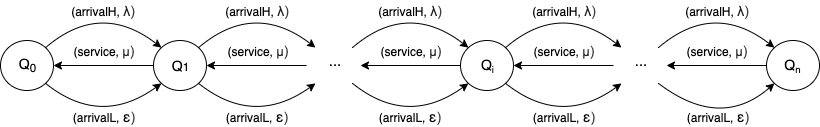
\includegraphics[width=1.0\textwidth]{queue-derivation-graph.png}
    \caption{Queue PEPA derivation graph}
    \label{fig:queue-derivation-graph}
\end{figure}

\subsection{Arrival Stream PEPA Component}

The \textit{Arrival Stream} PEPA component of the system is defined as follows:

\begin{align*} 
    Arrival_{high} &\defeq (arrivalH, \lambda).Arrival_{high} + (highPeriodEnd, \beta). Arrival_{low} \\
    Arrival_{low} &\defeq (arrivalL, \epsilon).Arrival_{low} + (lowPeriodEnd, \gamma). Arrival_{high}
\end{align*} 

\noindent Meaning that whenever the arrival rate is set in either \textit{high} or \textit{low}, the system will remain in its current state until that specific period ends and the system will adjust itself by using the switching operations \textit{highPeriodEnd} or \textit{lowPeriodEnd} accordingly.\newline

\par\noindent The previously described \textit{arrival stream} PEPA component can be also  graphically represented by the following derivation graph:

\begin{figure}[H]
    \centering
    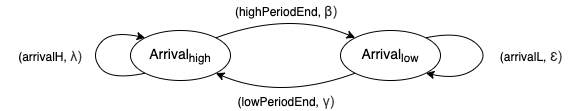
\includegraphics[width=1.0\textwidth]{arrival-stream-derivation-graph.png}
    \caption{Arrival Stream PEPA derivation graph}
    \label{fig:arrival-stream-derivation-graph}
\end{figure}

\subsection{Server PEPA Component}

The \textit{Server} PEPA component of the system is defined as follows:

\begin{align*} 
    ServerPowering_{on} &\defeq (powerup, \eta*(1 - \rho)).Server_{on} + (powerup, \eta * \rho).Server_{failOn} \\
    Server_{on} &\defeq (service, \mu).Server_{on} + (highPeriodEnd, \beta).ServerPowering_{off} \\
    ServerPowering_{off} &\defeq (poweroff, \xi*(1 - \rho)).Server_{off} + (poweroff, \xi * \rho).Server_{failOff} \\
    Server_{off} &\defeq (lowPeriodEnd, \gamma).ServerPowering_{on}
\end{align*}

\begin{align*}
    Server_{static} &\defeq (service, \mu).Server_{static} \\
    Server_{failOn} &\defeq (repair, \sigma).Server_{on} \\
    Server_{failOff} &\defeq (repair, \sigma).Server_{off}
\end{align*}

\noindent The presented states definitions illustrate the normal flow between all the possible server's states.\newline
To point out that we defined \(\rho\) as the probability that an error occurs during the execution of the \textit{powerup} and/or \textit{poweroff} activities.\newline

\par\noindent The previously described \textit{server} PEPA component can be also  graphically represented by the following derivation graphs:

\begin{figure}[H]
    \centering
    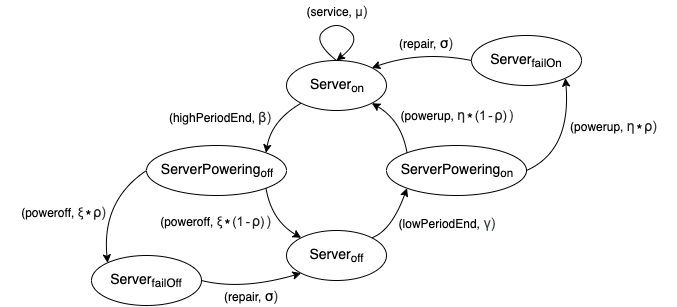
\includegraphics[width=1.0\textwidth]{server-derivation-graph.png}
    \caption{Server PEPA derivation graph}
    \label{fig:server-derivation-graph}
\end{figure}

\begin{figure}[H]
    \centering
    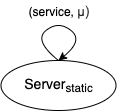
\includegraphics[width=2.5cm]{server-static-derivation-graph.png}
    \caption{Static server PEPA derivation graph}
    \label{fig:server-static-derivation-graph}
\end{figure}

%%%%%%%%%%%%%% 5 ENTIRE SYSTEM EXPRESSED IN PEPA %%%%%%%%%
\section{Entire System Expressed in PEPA}

The entire system in the PEPA process algebra is defined as follows:

\[System \defeq ((Arrival_{high} \underset{K}{\newbowtie}
 Server_{on} \underset{K}{\newbowtie} ... \underset{K}{\newbowtie} Server_{on}) \underset{Z}{\newbowtie} Server_{static}[M]) \underset{L}{\newbowtie} Q_{0}\]
 
\noindent Where respectively the sets \(K,Z,L\) are defined as follows:
 
\begin{itemize}
    \item \(K = \{highPeriodEnd\}\);
    \item \(Z = \emptyset \);
    \item \(L = \emptyset \).
\end{itemize}

\noindent Just to recall, the number of '\textit{\(Server_{on}\)}' present on the '\textit{System}' PEPA definition are equals to \(N - M\), where \(N\) are the total number of servers and \(M\) are the static ones.\newline

\par\noindent So, for example if we choose \(N = 6\) and \(M = 3\), we are considering a system with a total of 6 servers, in which 3 of them are static and the other 3 are dynamic.\newline
So, given those specifications the system PEPA definition is defined as follows:

\[System \defeq ((Arrival_{high} \underset{K}{\newbowtie}
 Server_{on} \underset{K}{\newbowtie} Server_{on} \underset{K}{\newbowtie}
 Server_{on}) \underset{Z}{\newbowtie} Server_{static}[M]) \underset{L}{\newbowtie} Q_{0}\]
 
\noindent In which \(K = \{highPeriodEnd\}, Z = L = \emptyset\) and \(M = 3\).

%%%%%%%%%%%% 6 DERIVATION GRAPH OF THE SYSTEM %%%%%%%%%%%
\section{Derivation Graph of the System}
\label{sec:derivation-graph-of-the-system}

The simplest way to represent the Markov Process underlying the PEPA model is in terms of its state transition diagram, which can be derived from the model's derivation graph.\newline

\par\noindent The derivation graph related to the considered system grows, in terms of components a therefore in its complexity, very fast due to the presence of many states involved in the system definition, so for simplicity we are going to consider only a sub-part of the entire system. Just for prospective, considering just one static server, one dynamic server and a queue component of length 2 would result in a 36 states system. For this reason we decided to analyse just the interaction between the components \(Arrival_{high}\) and \(Server_{on}\) as defined by the following PEPA equation: 

\[Arrival_{high} \underset{\{highPeriodEnd\}}{\newbowtie} Server_{on} \]

\noindent This generates a 12 states diagram as summarized in the following image:

\begin{figure}[H]
    \centering
    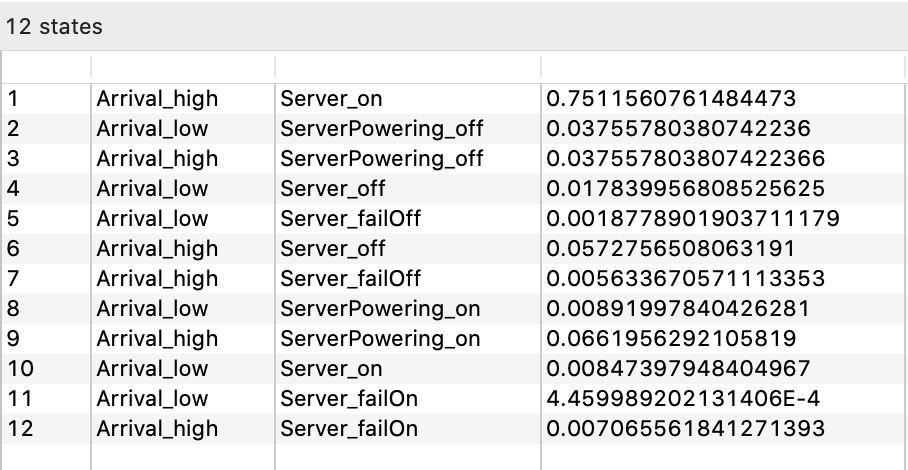
\includegraphics[width=10.5cm]{space-state-view.png}
    \caption{Space state view for the system equation - PEPA Eclipse plug-in}
    \label{fig:space-state-view}
\end{figure}

\noindent For readability reasons the provided derivation graph (Figure \ref{fig:sub-system-derivation-graph}) will have in each node a number corresponding to the associated states row present in 'Figure \ref{fig:space-state-view}'.\newline

\par\noindent The derivation graph for the considered PEPA equation is illustrated as follows:

\begin{figure}[H]
    \centering
    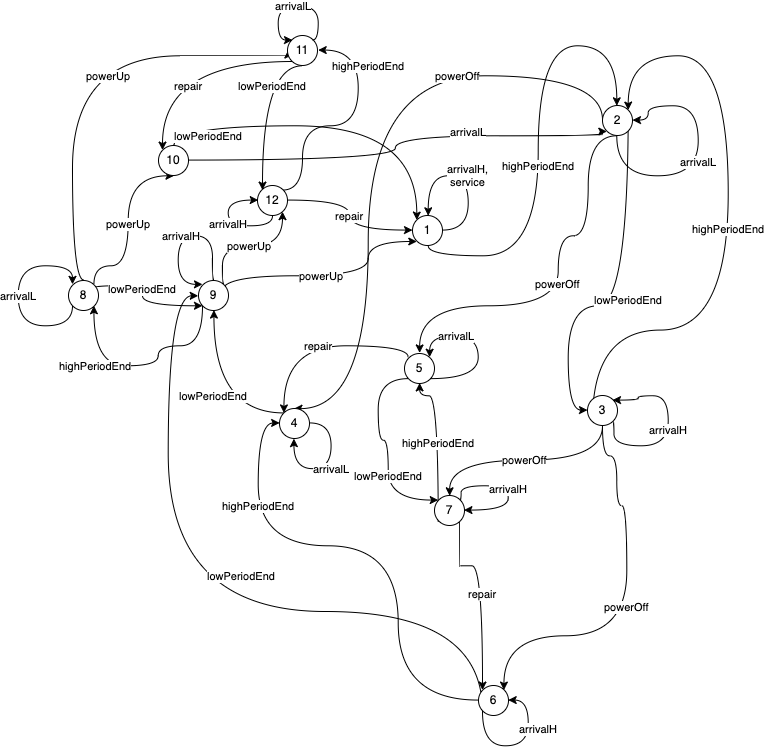
\includegraphics[width=1.0\textwidth]{sub-system-derivation-graph.png}
    \caption{Sub-system derivation graph}
    \label{fig:sub-system-derivation-graph}
\end{figure}

\begin{figure}[H]
    \centering
    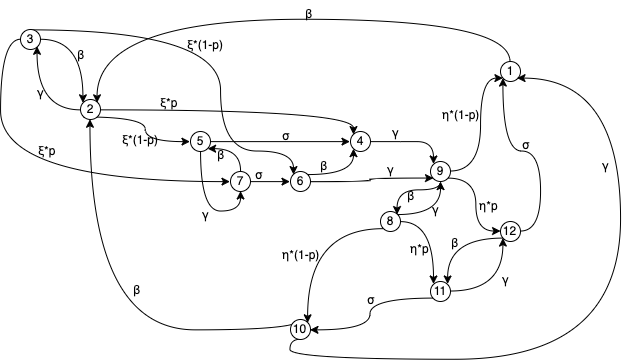
\includegraphics[width=1.0\textwidth]{CTMC-graph.png}
    \caption{Continuous Time Markov Chain graph}
    \label{fig:CTMC-graph}
\end{figure}
 
%%%%%%%%%%%%%% 7 INFINITESIMAL GENERATOR MATRIX %%%%%%%%%% 
\section{Infinitesimal Generator Matrix}

In this section we are going to present the infinitesimal generator matrix \(Q\) of the Markov process associated to the previous described components' subset of the system (\autoref{sec:derivation-graph-of-the-system}).\newline

\par\noindent For space and complexity reasons (\(|S| = 12\)) we will not report the associated \textit{Continuous Time Markov Chain} representation graph for the chosen components' subset.\newline

\par\noindent Just to recall, the \textit{infinitesimal generator matrix} is constructed such that for every element \(q_{ij}\) (with \(i \neq j\), where \(i,j\) start from 1 up to the number of states involved) denotes the rate departing from \(i\) and arriving in state \(j\) (if there are multiple arrow starting from \(i\) and arriving in \(j\), just consider the sum of the rates). Meanwhile the diagonal elements \(q_{ii}\) are defined such that:

\[q_{ii} = - \sum_{j \neq i} q_{ij}\]

\noindent The infinitesimal  generator  matrix associated to the analyzed components is defined as follows:

{   
\fontsize{3pt}{8pt}\selectfont 
\[Q =
\setcounter{MaxMatrixCols}{12}
\begin{bmatrix}
    -\beta & \beta & 0 & 0 & 0 & 0 & 0 & 0 & 0 & 0 & 0 & 0 \\
    0 & -(\gamma + \xi) & \gamma & \xi * (1 - \rho) & \xi * \rho & 0 & 0 & 0 & 0 & 0 & 0 & 0 \\
    0 & \beta & -(\beta + \xi) & 0 & 0 & \xi * (1 - \rho) & \xi * \rho & 0 & 0 & 0 & 0 & 0 \\
    0 & 0 & 0 & -\gamma & 0 & 0 & 0 & 0 & \gamma & 0 & 0 & 0 \\
    0 & 0 & 0 & \sigma & -(\sigma + \gamma) & 0 & \gamma & 0 & 0 & 0 & 0 & 0 \\
    0 & 0 & 0 & \beta & 0 & -(\beta + \gamma) & 0 & 0 & \gamma & 0 & 0 & 0 \\
    0 & 0 & 0 & 0 & \beta & \sigma & -(\beta + \sigma) & 0 & 0 & 0 & 0 & 0 \\
    0 & 0 & 0 & 0 & 0 & 0 & 0 & -(\gamma + \eta) & \gamma & \eta * (1 - \rho) & \eta * \rho & 0 \\
    \eta * (1 - \rho) & 0 & 0 & 0 & 0 & 0 & 0 & \beta & -(\beta + \eta) & 0 & 0 & \eta * \rho \\
    \gamma & \beta & 0 & 0 & 0 & 0 & 0 & 0 & 0 & -(\beta + \gamma) & 0 & 0 \\
    0 & 0 & 0 & 0 & 0 & 0 & 0 & 0 & 0 & \sigma & -(\sigma + \gamma) & \gamma \\
    \sigma & 0 & 0 & 0 & 0 & 0 & 0 & 0 & 0 & 0 & \beta & -(\sigma + \beta)
\end{bmatrix}\]
}

{   
\fontsize{3pt}{8pt}\selectfont 
\[Q^{T}_{N} =
\setcounter{MaxMatrixCols}{12}
\begin{bmatrix}
    -\beta & 0 & 0 & 0 & 0 & 0 & 0 & 0 & \eta * (1 - \rho) & \gamma & 0 & \sigma \\
    \beta & -(\gamma + \xi) & \beta & 0 & 0 & 0 & 0 & 0 & 0 & \beta & 0 & 0 \\
    0 & \gamma & -(\beta + \xi) & 0 & 0 & 0 & 0 & 0 & 0 & 0 & 0 & 0 \\
    0 & \xi * (1 - \rho) & 0 & -\gamma & \sigma & \beta & 0 & 0 & 0 & 0 & 0 & 0 \\
    0 & \xi * \rho & 0 & 0 & -(\sigma + \gamma) & 0 & \beta & 0 & 0 & 0 & 0 & 0 \\
    0 & 0 & \xi * (1 - \rho) & 0 & 0 & -(\beta + \gamma) & \sigma & 0 & 0 & 0 & 0 & 0 \\
    0 & 0 & \xi * \rho & 0 & \gamma & 0 & -(\beta + \sigma) & 0 & 0 & 0 & 0 & 0 \\
    0 & 0 & 0 & 0 & 0 & 0 & 0 & -(\gamma + \eta) & \beta & 0 & 0 & 0 \\
    0 & 0 & 0 & \gamma & 0 & \gamma & 0 & \gamma & -(\beta + \eta) & 0 & 0 & 0 \\
    0 & 0 & 0 & 0 & 0 & 0 & 0 & \eta * (1 - \rho) & 0 & -(\beta + \gamma) & \sigma & 0 \\
    0 & 0 & 0 & 0 & 0 & 0 & 0 & \eta * \rho & 0 & 0 & -(\sigma + \gamma) & \beta \\
    1 & 1 & 1 & 1 & 1 & 1 & 1 & 1 & 1 & 1 & 1 & 1 \\
\end{bmatrix}\]
}

%%%%%%%%%%%% 8 EVALUATION %%%%%%%%%%%%%%
\section{Evaluation}

\subsection{Global Balance Equations}

In this section we are going to present how to calculate the \textit{global balance equation}, but we are not presenting the actual calculation due to complexity reasons.\newline

\par\noindent Just to remind that finding the \textit{global balance equation} means calculating the following formula:

\[\pi Q = 0\]

\noindent Moreover, since the previously presented state space had 12 states, the global balance equations will have \(12 + 1\) equations (the \(13^{th}\) one is the normalization condition) in 12 unknowns as represented below:

\begin{equation*}
  \begin{cases}
    \pi_{1} \cdot \beta = \pi_{9} \cdot (\eta \cdot (1 - \rho)) + \pi_{10} \cdot \gamma + \pi_{12} \cdot \sigma \\
    \pi_{2} \cdot (\gamma + \xi) = \pi_{1} \cdot \beta + \pi_{3} \cdot \beta + \pi_{10} \cdot \beta \\
    \pi_{3} \cdot (\beta + \xi) = \pi_{2} \cdot \gamma \\
    \pi_{4} \cdot \gamma = \pi_{2} \cdot (\xi \cdot (1 - p)) + \pi_{5} \cdot \sigma + \pi_{6} \cdot \beta \\
    \pi_{5} \cdot (\sigma + \gamma) = \pi_{2} \cdot (\xi \cdot \rho) + \pi_{7} \cdot \beta \\
    \pi_{6} \cdot (\beta + \gamma) = \pi_{3} \cdot (\xi \cdot (1 - \rho)) +\pi_{7} \cdot \sigma \\
    \pi_{7} \cdot (\beta + \sigma) = \pi_{3} \cdot (\xi \cdot \rho) + \pi_{5} \cdot \gamma \\
    \pi_{8} \cdot (\gamma + \eta) = \pi_{9} \cdot \beta \\
    \pi_{9} \cdot (\beta + \eta) = \pi_{4} \cdot \gamma + \pi_{6} \cdot \gamma + \pi_{8} \cdot \gamma \\
    \pi_{10} \cdot (\beta + \gamma) = \pi_{8} \cdot (\xi \cdot (1 - \rho)) + \pi_{11} \cdot \sigma \\
    \pi_{11} \cdot (\sigma + \gamma) = \pi_{8} \cdot (\xi \cdot \rho) + \pi_{12} \cdot \beta \\
    \pi_{12} \cdot (\sigma + \beta) = \pi_{9} \cdot (\xi \cdot \rho) + \pi_{11} \cdot \gamma \\
    \pi_{1} + \pi_{2} + \pi_{3} + \pi_{4} + \pi_{5} + \pi_{6} + \pi_{7} + \pi_{8} + \pi_{9} + \pi_{10} + \pi_{11} + \pi_{12} = 1
  \end{cases}
\end{equation*}

\noindent So, once the above system equations is resolved, i.e. you find out the values for each \(\pi_{i}\) for \(i=1, ... , 12\), those values will tell you the portion of time, expressed in probability, that the system behaves like the \(\pi_{i}\) components/state.

\subsection{Sojourn Time}

The dynamic behaviour of the system is represented by the transitions between its states and the times spent in states: the sojourn times. The sojourn times are memoryless.\newline

\par\noindent Just to recall, the \textit{exit rate} from a component \(P\) is the rate at which the system leaves the state corresponding to the component \(P\).\newline
So, regarding our sub-system, the various \textit{exit rates} are:

\begin{align*}
    q(1) &= \beta \\
    q(2) &= \gamma + \xi \\
    q(3) &= \beta + \xi \\
    q(4) &= \gamma \\
    q(5) &= \sigma + \gamma \\
    q(6) &= \beta + \gamma \\
    q(7) &= \beta + \sigma \\
    q(8) &= \sigma + \eta \\
    q(9) &= \beta + \eta \\
    q(10) &= \beta + \gamma \\
    q(11) &= \sigma + \gamma \\
    q(12) &= \sigma + \beta \\
\end{align*}

\noindent Now that we have all the various \textit{exit rates} we can calculate the \textit{sojourn time} for each state. As before, we recall that the \textit{sojourn time} of a component \(P\) is equals to \(ST(p) = (q(p))^{-1}\), where \(q(p)\) identifies the exit rate of the component '\(p\)'.\newline

\par\noindent The relative \textit{sojourn times} of the analyzed sub-part of the system are presented below:

\begin{align*}
    ST(1) &= \frac{1}{\beta} \\
    ST(2) &= \frac{1}{\gamma + \xi} \\
    ST(3) &= \frac{1}{\beta + \xi} \\
    ST(4) &= \frac{1}{\gamma} \\
    ST(5) &= \frac{1}{\sigma + \gamma} \\
    ST(6) &= \frac{1}{\beta + \gamma} \\
    ST(7) &= \frac{1}{\beta + \sigma} \\
    ST(8) &= \frac{1}{\sigma + \eta} \\
    ST(9) &= \frac{1}{\beta + \eta} \\
    ST(10) &= \frac{1}{\beta + \gamma} \\
    ST(11) &= \frac{1}{\sigma + \gamma} \\
    ST(12) &= \frac{1}{\sigma + \beta} \\
\end{align*}

\subsection{Utilisation}

The \textit{utilisation} measure is the total probability that the model is in one of the states in which the resource is in use.\newline
\noindent So, regarding our sub-set of the system the utilization variables are reported below:

\[U_{Arrival_{high}} = \pi_{1} + \pi_{3} + \pi_{6} + \pi_{7} + \pi_{9} + \pi_{12}\]

\[U_{Server_{on}} = \pi_{1} + \pi_{10}\]

\section{Evaluation of the System Using the PEPA Eclipse Plug-In}
In this final section we have modeled our entire system using the PEPA Eclipse plug-in in order to examine and extrapolate further meaningful information that there will be presented below.\newline

\par\noindent First of all, the system expressed using the PEPA plug-in is equals to the following snippet of code:

\begin{lstlisting}[caption=PEPA Eclipse Plug-In of the System]
l = 50.0;
e = 10.0;
m = 10.0;
b = 10.0;
g = 10.0;
n = 100.0;
r = 0.1;
x = 100.0;
s = 1.0;

Q0 = (arrivalH,l).Q1 + (arrivalL,e).Q1;
Q1 = (arrivalH,l).Q2 + (arrivalL,e).Q2 + (service,m).Q0;
Q2 = (service,m).Q1;

Arrival_high = (arrivalH,l).Arrival_high + (highPeriodEnd,b).Arrival_low;
Arrival_low = (arrivalL,e).Arrival_low + (lowPeriodEnd,g).Arrival_high; 

ServerPowering_on = (powerup, n * (1-r)).Server_on + (powerup, n*r).Server_failOn;
Server_on = (service,m).Server_on + (highPeriodEnd,b).ServerPowering_off;
ServerPowering_off = (poweroff,x*(1-r)).Server_off + (poweroff,x*r).Server_failOff;
Server_off = (lowPeriodEnd,g).ServerPowering_on;

Server_static = (service,m).Server_static;
Server_failOn = (repair,s).Server_on;
Server_failOff = (repair,s).Server_off;

((Arrival_high <highPeriodEnd> Server_on <highPeriodEnd> Server_on <highPeriodEnd> Server_on) <> Server_static <> Server_static <> Server_static ) <> Q0
\end{lstlisting}

\noindent To point out that we have modeled a system having \(N = 6\) servers, which 3 of them are \textit{dynamic} and the rest are \textit{static} (i.e. always on).\newline
For complexity reasons the queue capacity has been bounded at 2.\newline
Finally the various rates were set as follows:

\begin{itemize}
    \item \textbf{High arrival rate}: 50;
    \item \textbf{Low arrival rate}: 10;
    \item \textbf{Powering-up and down}: 100 in equally \textit{high} and \textit{low} period of job arrivals.
\end{itemize}

\noindent Using this specific system configuration on the plug-in environment, we retrieved the \textbf{throughput} as illustrated in the following image:

\begin{figure}[H]
    \centering
    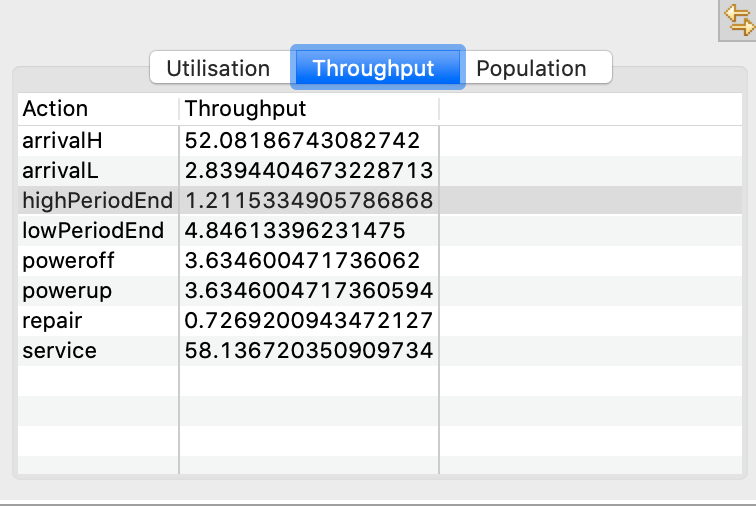
\includegraphics[width=10.5cm]{throughput-table.png}
    \caption{Throughput evaluation of the system}
    \label{fig:throughput-table}
\end{figure}

\begin{figure}[H]
    \centering
    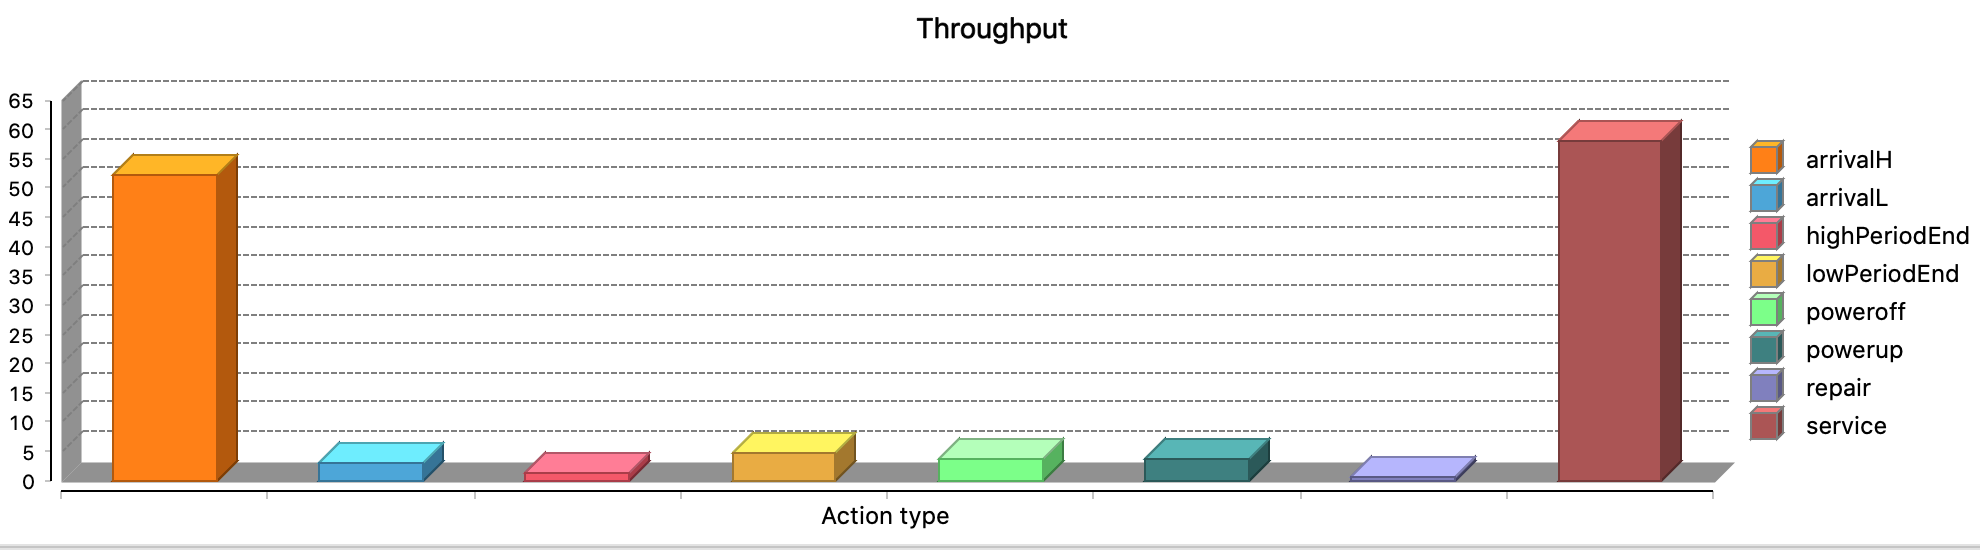
\includegraphics[width=16.5cm]{throughput-graph.png}
    \caption{Throughput evaluation of the system}
    \label{fig:throughput-graph}
\end{figure}

\noindent Moreover, in the following images you can appreciate the \textbf{utilization} regarding the various system's states.

\begin{figure}[H]
    \centering
    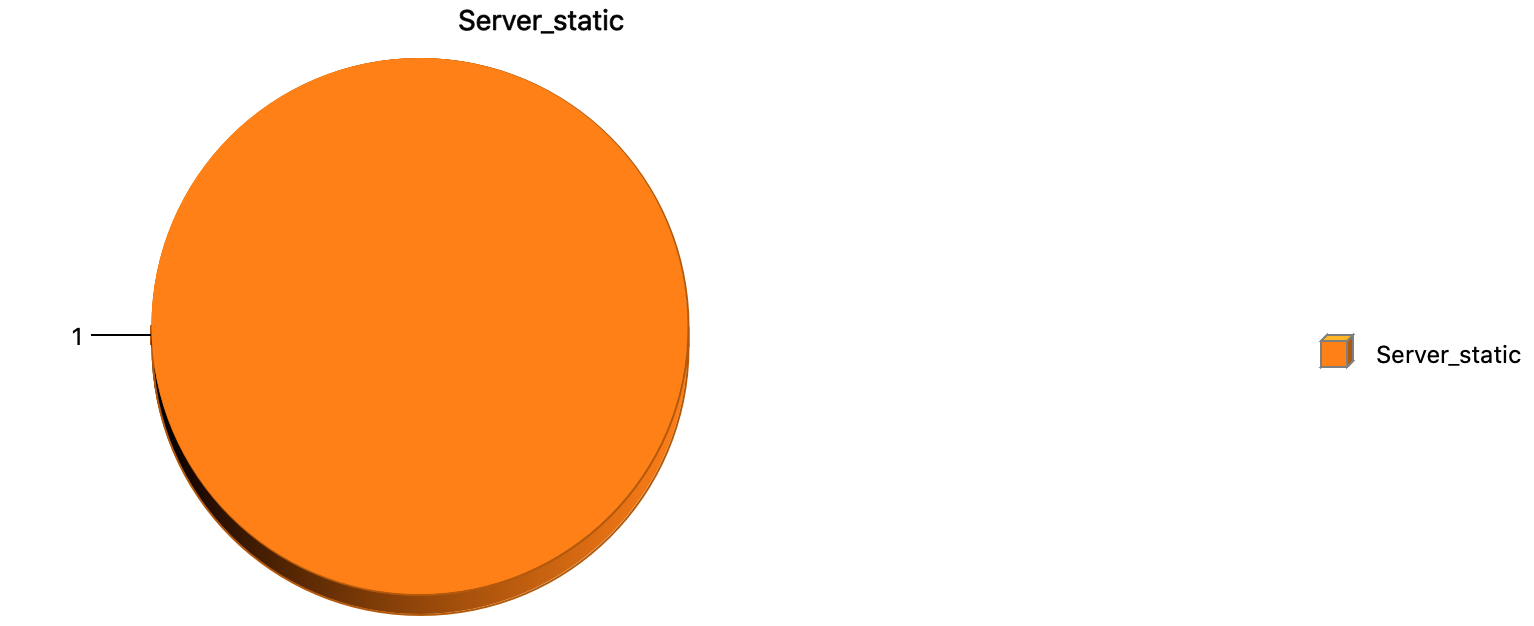
\includegraphics[width=16.5cm]{utilisation-static-server.png}
    \caption{Utilisation Static Server component}
    \label{fig:utilisation-static-server}
\end{figure}

\begin{figure}[H]
    \centering
    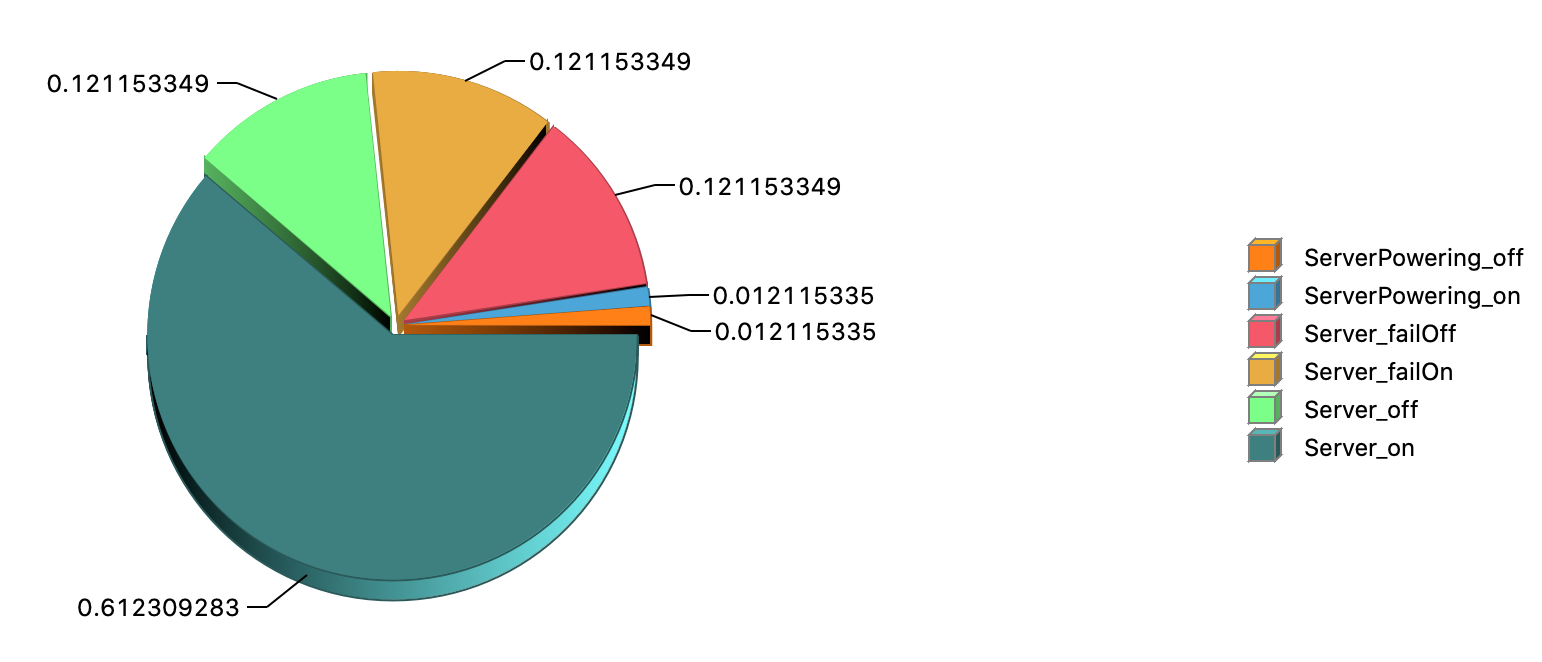
\includegraphics[width=16.5cm]{utilisation-dynamic-server.png}
    \caption{Utilisation Dynamic Server component}
    \label{fig:utilisation-dynamic-server}
\end{figure}

\begin{figure}[H]
    \centering
    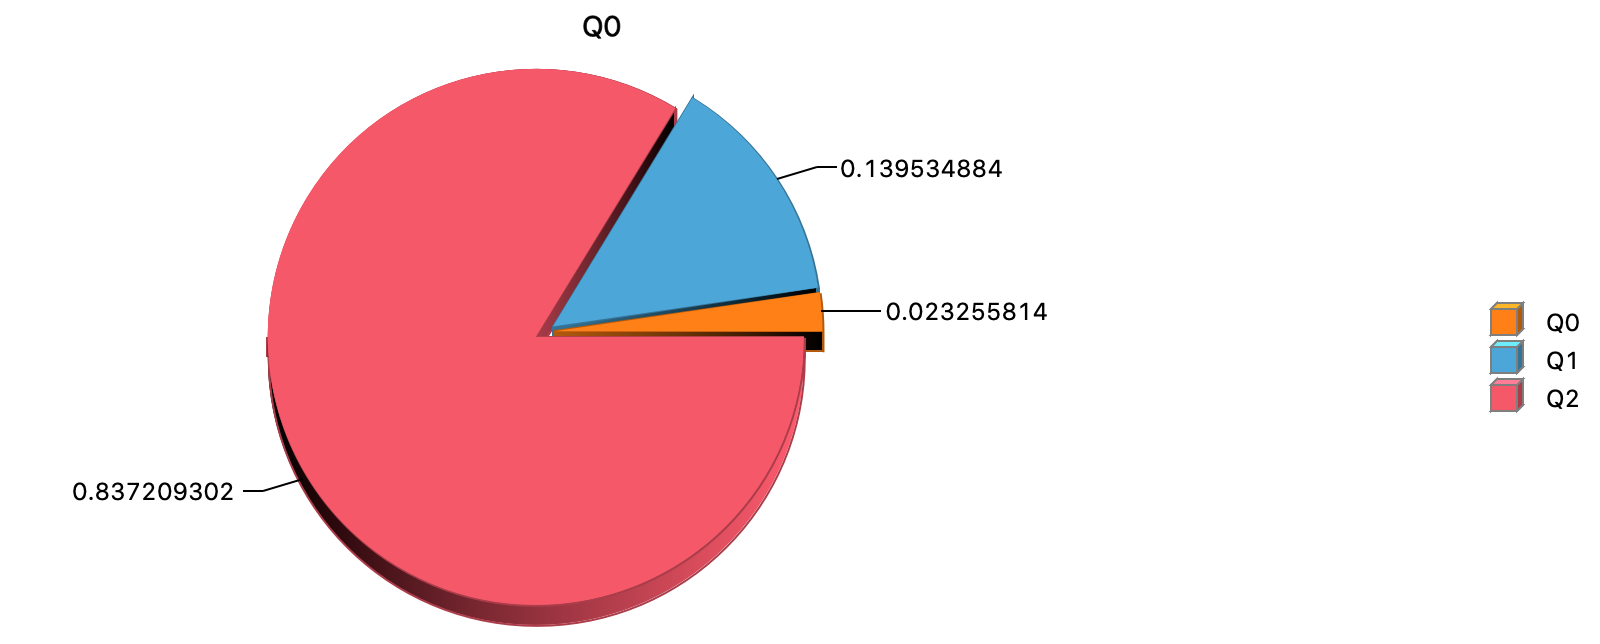
\includegraphics[width=16.5cm]{utilisation-queue.png}
    \caption{Utilisation Queue component}
    \label{fig:utilisation-queue}
\end{figure}

\noindent Finally in the following image it will be presented the \textbf{population} for the considered system's configuration.

\begin{figure}[H]
 \centering
    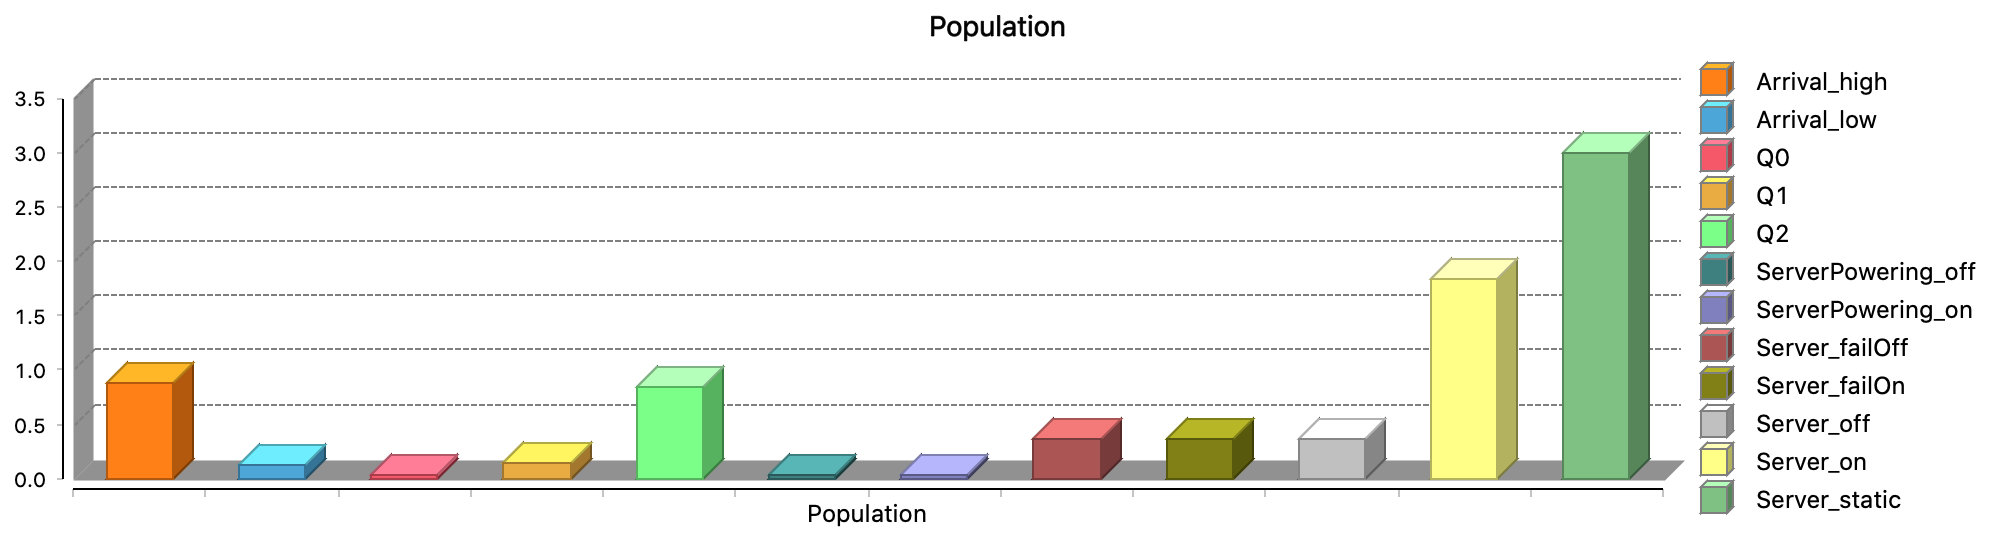
\includegraphics[width=16.5cm]{population-graph.png}
    \caption{Population for a 3 dynamic + 3 static servers configuration}
    \label{fig:population-graph}
\end{figure}

\newpage
\bibliographystyle{plain}
\raggedright
\bibliography{refs}

\end{document}